\begin{figure}
    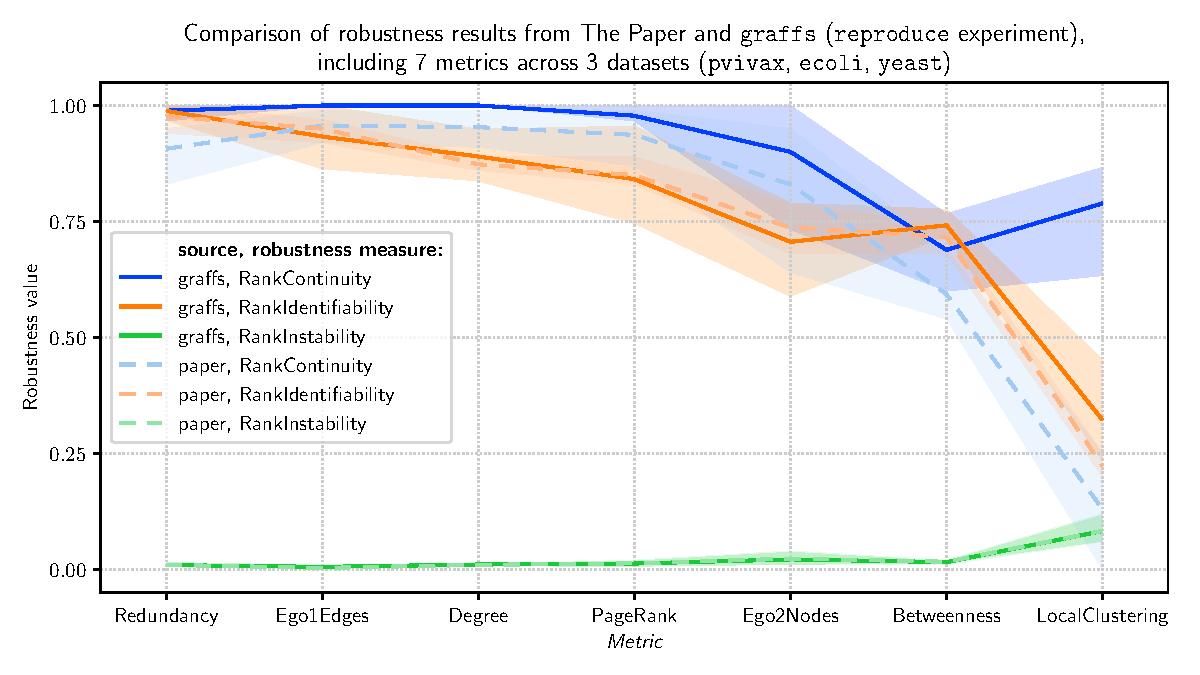
\includegraphics[width=\linewidth]{plot_reproduction.pdf}
    \vspace*{-0.6cm}
    \caption{Comparison of results from The Paper and \graffs.
    Each color corresponds to one robustness measure.
    Bands show the range of measured values across the 3 datasets, and lines show the average.
    Solid and dashed bands correspond to results obtained by \graffs and The Paper, respectively.}
    \label{fig:plot_reproduction}
    \footnotesize
    \begin{flushleft}
        Note that high values of RankContinuity and RankIdentifiability mean high robustness, whereas high values of RankInstability mean low robustness.
        Metrics are sorted from left to right by their decreasing combined robustness.
    \end{flushleft}
\end{figure}
